\chapter{エントロピーと通信容量}
次に通信容量について説明する。
通信容量は、通信路で伝達できる最大の($1$記号当りの)情報量のことである。
通信容量$C$はこのようにして計算することができる。
$$
C=\max_{P_X}I(X;Y)
$$
ここで、$\max_{P_X}$は先験確率$P_X$を動かして最大値を求めることを意味している。
すなわち通信容量は相互情報量I(X;Y)を$P_X$で最大化したものとなっている。相互情報量は、出力$Y$を知ったときに得る$X$に関する情報量のことで、通信路で伝達される情報量を表している。



相互情報量について詳しく見るために、エントロピーについて説明をする。
エントロピーとはXに関する曖昧さを表す量で、このような式で計算することができる。
$$
H(X)=-\sum_xP_X(x)\log P_X(x)
$$
条件付きエントロピーは、
$Y$の値を知った時に$x$に関して残る平均の曖昧さを表す量で、
このような式で計算することができる。
$$
H(X|Y)=\sum_xP_Y(y)H(X|Y=y)$$
$$
H(X|Y=y)=-\sum_xP(x|y)\log P(X|Y)
$$




相互情報量は、エントロピーから条件付きエントロピーを引いたもののことでこのように表される。
$$
I(X;Y)=H(X)-H(X|Y)
$$
さきほど説明したように、エントロピー$H(X)$は、Xに関する曖昧さを表しており、
条件付きエントロピー$H(X|Y)$は、$Y$の値を知った時に$x$に関して残る平均の曖昧さ
を表している。したがって$H(X)$から$H(X|Y)$を引くとYの値を知ることにより、消えた$X$の曖昧さになる。
すなわちこれは、出力$Y$を知ったときに得る$X$に関する情報量となっている。
\figref{Fig3_1}は相互情報量とエントロピーの関係を表している。


    \begin{figure}[H]
        \centering   
        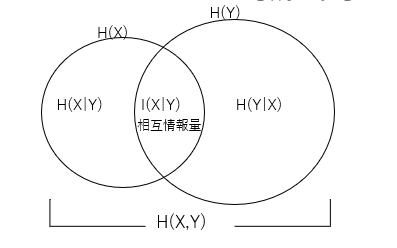
\includegraphics[width=0.7\textwidth]{img/Fig2.png}
        \caption[sample image (png)]{相互情報量とエントロピーの関係}
        \label{Fig3_1}
    \end{figure}


$H(X)$から$H(X|Y)$を引くと相互情報量$I(X|Y)$となるが、
$H(Y)$から$H(Y|X)$を引いても相互情報量$I(X|Y)$が得られることが知られている。


次に2元対称通信路の通信容量について計算する。
さきほど説明したように、通信容量は以下の式で計算することができる。
$$
C=\max_{P_X}I(X;Y)
$$
ここで、最適な$P_X$は、$P_X(0)=P_X(1)=1/2$となることが知られているので、
この事実を使って通信容量を計算することにする。
このとき、$P_Y(0)=P_Y(1)$を計算すると$1/2$となる。
また、エントロピー$H(Y)$は$1$となり、条件付きエントロピーは
$$
-p\log_2p-(1-p)\log_2(1-p)
$$
となる。
よって通信容量$C$はこのように$p$を使って計算できる。

